% ===========================================================
% SECTION 4: EVALUATION AND DISCUSSION
% =====================================================================================

\section{Evaluation and Discussion}
\label{sec:evaluation}

\subsection{Dataset Overview}
\label{subsec:datasets}

We tested our approach across four diverse process mining datasets to validate cross-domain applicability:

\textbf{Traffic Fines (Government):} 150,370 cases with 561,470 events spanning 12 years. Represents long-term citizen interaction patterns with government processes including fine creation, payments, and appeals. We use the Road Traffic Fine Management Process event log, a widely used real-world dataset for process mining research \cite{deleoni2015traffic}.

\textbf{BPI Challenge 2012 (Finance):} 13,087 cases with 262,200 events from Dutch financial institution loan applications. Shows structured business workflow with moderate complexity and predictable timing patterns. The BPI Challenge 2012 event log is a standard benchmark in the process mining community for evaluating techniques on financial processes \cite{vandongen2012bpi}.

\textbf{BPI Challenge 2017 (Finance):} 31,509 cases with 1,202,267 events representing credit application processes. Demonstrates high-complexity financial workflows with the largest event volume in our test set.

\textbf{Sepsis Cases (Healthcare):} 1,050 cases with 15,214 events from hospital patient treatment. Exhibits time-critical medical decision patterns with urgent care requirements and concentrated timing distributions. Healthcare event logs, such as those described in \cite{rojas2016healthcare}, present unique challenges and opportunities for process mining analysis.

These datasets provide comprehensive coverage across government, finance, and healthcare domains with varying scales, complexity levels, and timing characteristics.

\subsection{Filtering Effectiveness}
\label{subsec:filtering_results}

Our filtering approach successfully removes case-start events while preserving meaningful patterns:

\begin{itemize}
    \item \textbf{Traffic Fines:} Removed 160,811 events (28.6\%) - highest reduction due to government process structure
    \item \textbf{BPI 2012:} Removed 13,087 events (5.0\%) - moderate reduction in structured financial process
    \item \textbf{BPI 2017:} Removed 31,509 events (2.6\%) - lowest reduction in complex financial workflow
    \item \textbf{Sepsis:} Removed 1,074 events (7.1\%) - moderate reduction in healthcare process
\end{itemize}

The filtering percentages correlate with process structure: simpler processes with clear start events show higher filtering rates, while complex processes with multiple initiation patterns show lower rates. All filtering preserved analytical validity as confirmed by manual inspection of the removed events.

\subsection{Cross-Domain Pattern Discovery}
\label{subsec:patterns}

Violin chart visualization revealed distinct timing patterns in each domain, as shown in Figure \ref{fig:cross_domain_patterns}.

\begin{figure}[H]
\centering
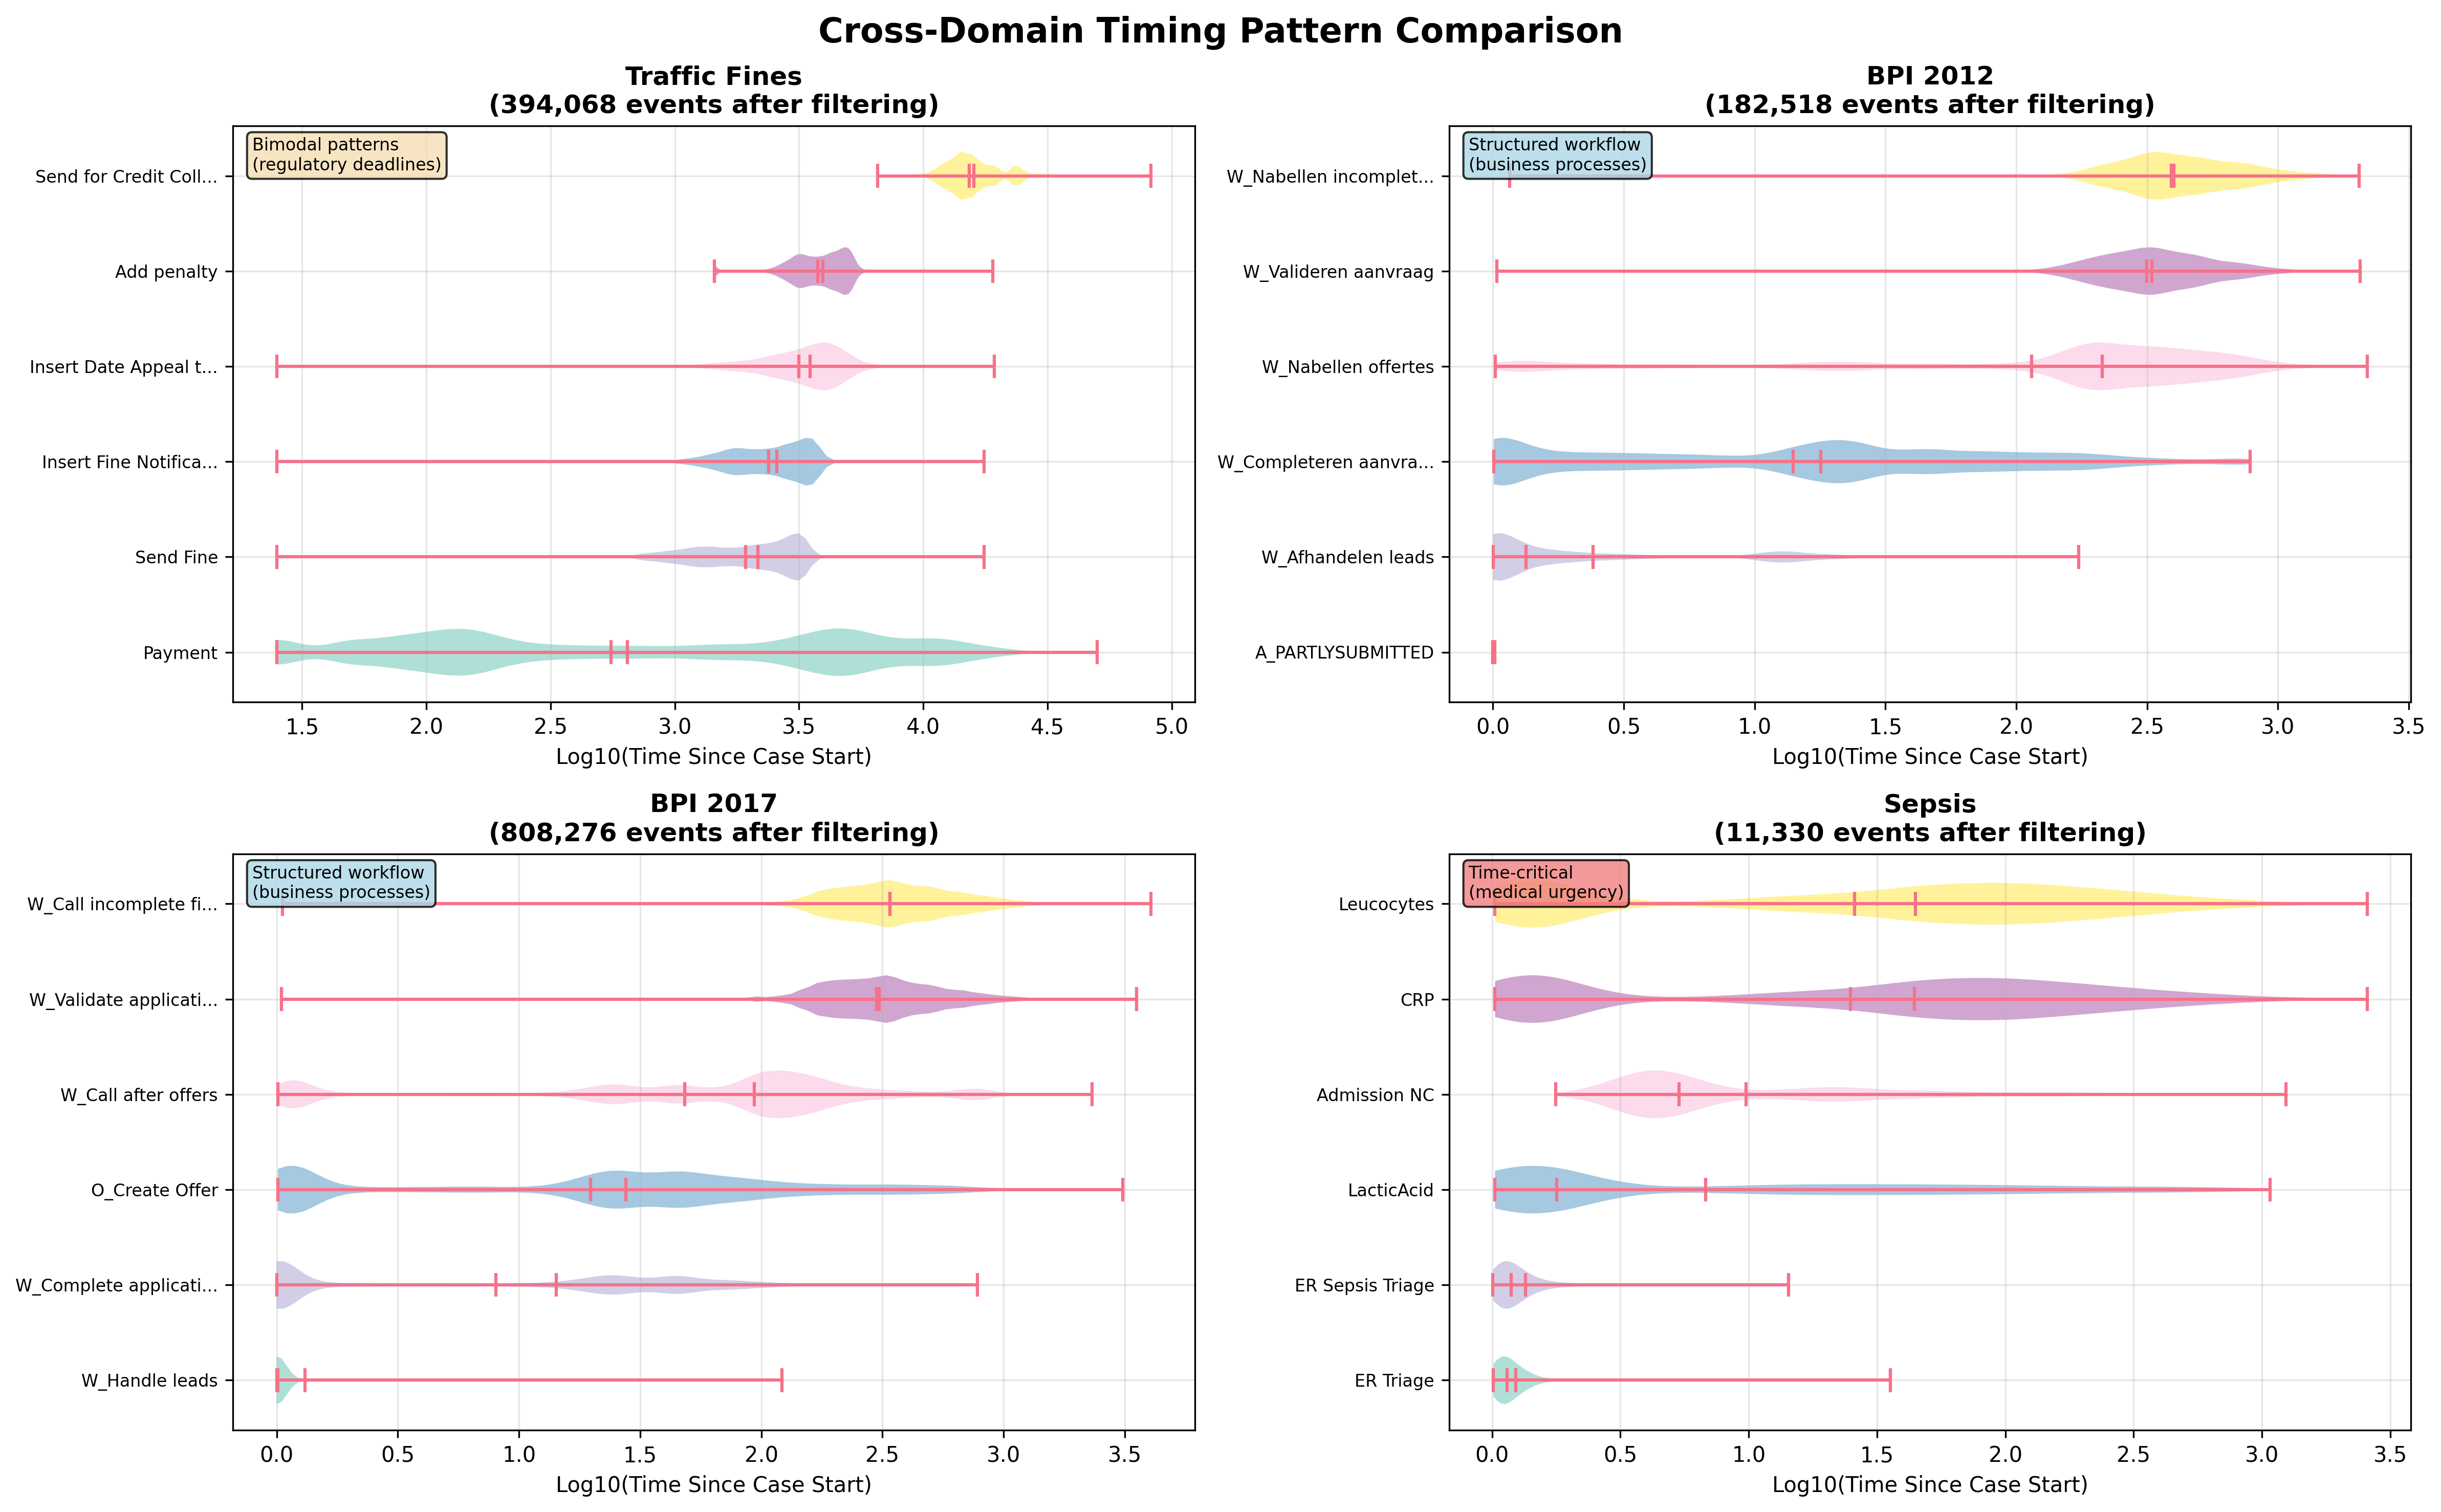
\includegraphics[width=\textwidth]{fig/cross_domain_patterns.png}
\caption{Cross-domain timing patterns revealed by violin charts. Each dataset shows distinct distribution characteristics: government processes exhibit bimodal patterns with regulatory deadlines, financial processes show structured workflow stages, and healthcare processes demonstrate time-critical clustering.}
\label{fig:cross_domain_patterns}
\end{figure}

\textbf{Government Processes (Traffic Fines):} Exhibited bimodal distributions with clear peaks at 30 days and 6 months, corresponding to payment deadlines and legal requirements. The patterns show strong correlation with regulatory timeframes and citizen behavior.

\textbf{Financial Processes (BPI Challenges):} Showed structured workflow stages with predictable timing intervals. BPI 2012 demonstrated consistent timing patterns reflecting standardized business procedures, while BPI 2017 showed higher variability due to increased process complexity.

\textbf{Healthcare Processes (Sepsis):} Demonstrated time-critical clustering with rapid initial responses within the first few hours, followed by gradual treatment progression. The urgent nature of medical care results in highly concentrated distributions reflecting clinical protocols.

These findings validate our hypothesis that different process domains exhibit distinct timing signatures that require flexible visualization approaches.

\subsection{Transformation Effectiveness}
\label{subsec:transformation_results}

Different transformations proved optimal for different dataset characteristics, as demonstrated in Figure \ref{fig:transformation_comparison}.

\begin{figure}[H]
\centering
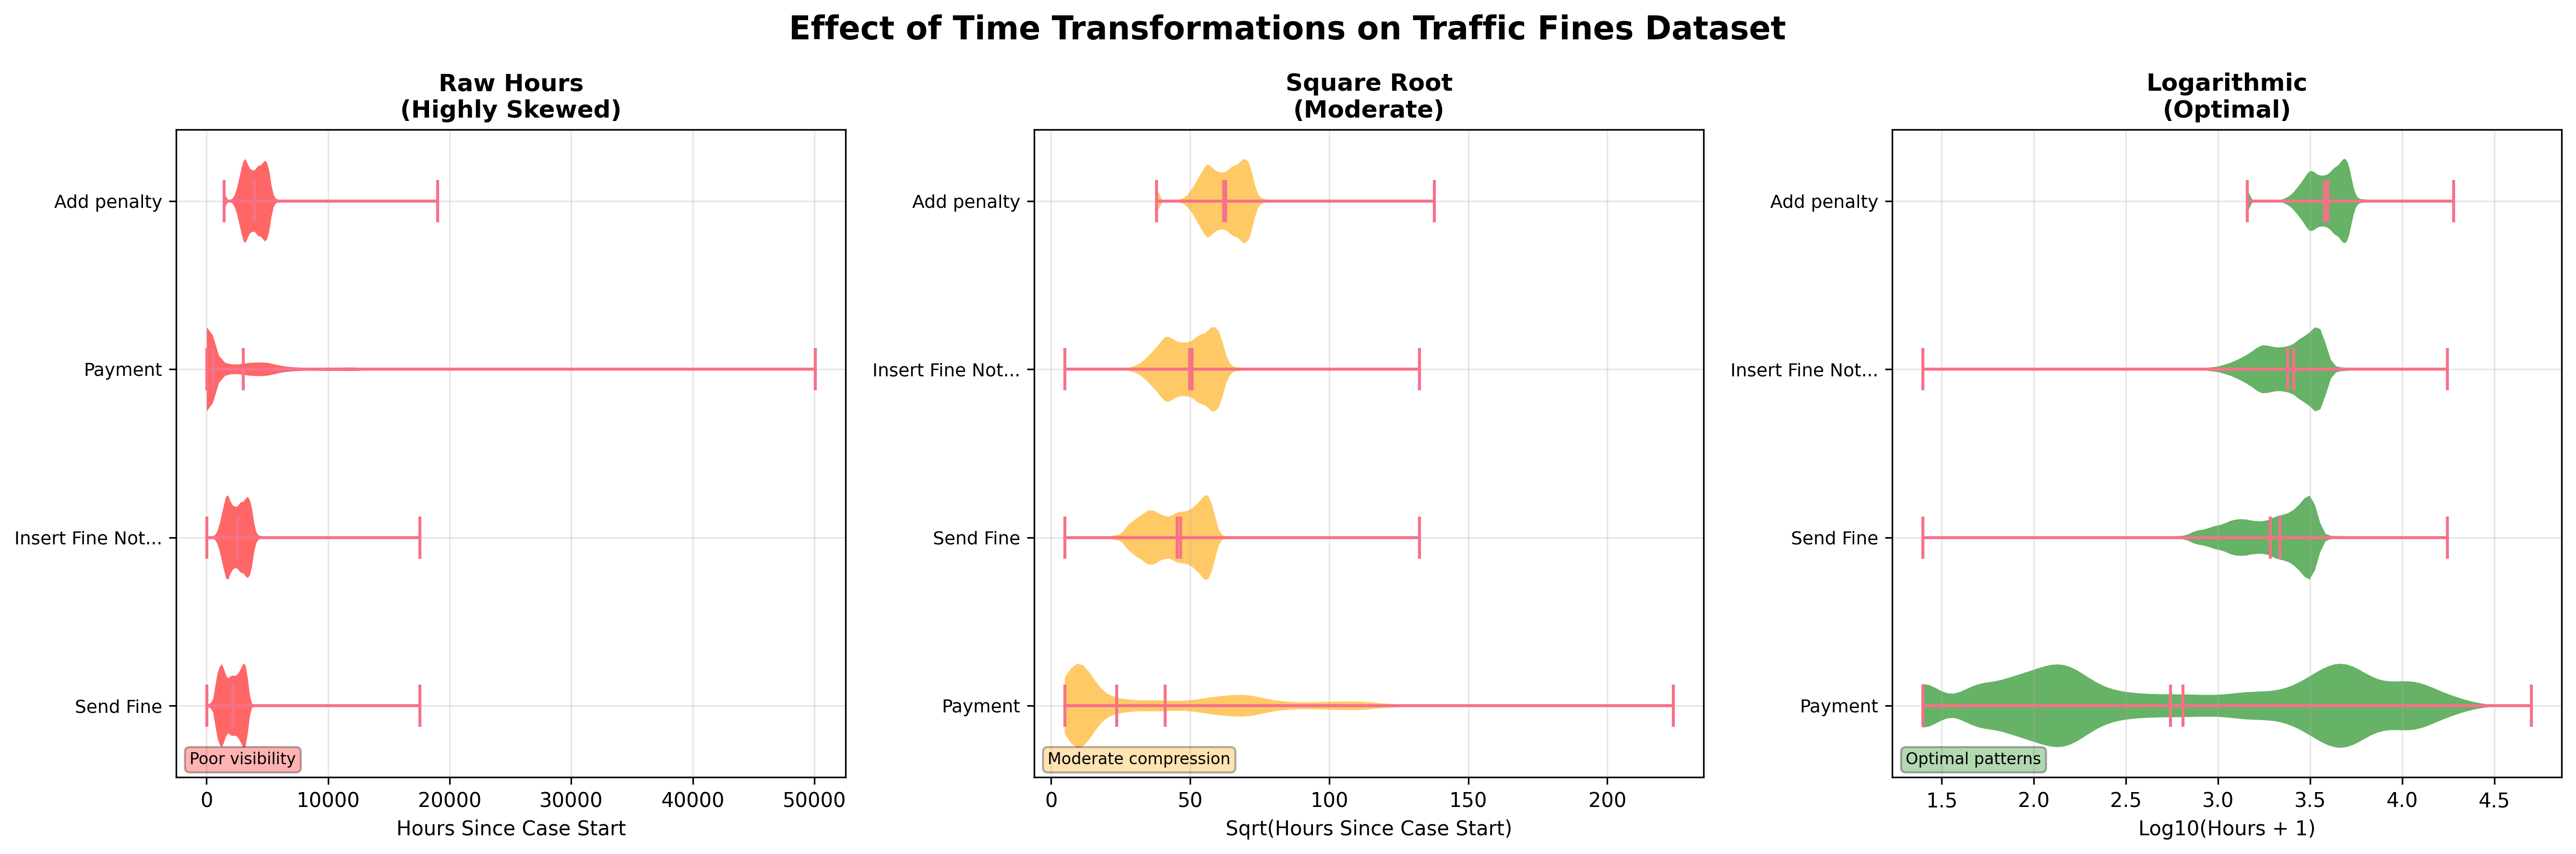
\includegraphics[width=\textwidth]{fig/transformation_comparison.png}
\caption{Effect of different time transformations on Traffic Fines dataset. Raw hours show extreme skewness, square root provides moderate compression, and logarithmic transformation reveals optimal pattern visibility for this highly skewed dataset.}
\label{fig:transformation_comparison}
\end{figure}

\textbf{Logarithmic Transformation:} Most effective for Traffic Fines and BPI datasets with extreme right-skewness spanning years or months. Successfully compressed long tails while preserving early-stage patterns.

\textbf{Raw Time Units:} Optimal for Sepsis dataset where absolute timing matters for clinical decisions. Hours and days provided meaningful clinical context that other transformations obscured.

\textbf{Square Root Transformation:} Provided good middle ground for BPI 2012 with moderate skewness. Balanced compression with pattern preservation for structured business workflows.

\textbf{Min-Max Scaling:} Enabled effective cross-dataset comparison by normalizing different time scales to comparable ranges. Essential for comparative analysis across domains.

No single transformation worked optimally for all datasets, confirming the need for multiple transformation options in our design.

\subsection{Visualization Insights}
\label{subsec:insights}

The violin chart approach revealed patterns invisible to traditional visualizations, as illustrated in Figure \ref{fig:violin_vs_traditional}.

\begin{figure}[H]
\centering
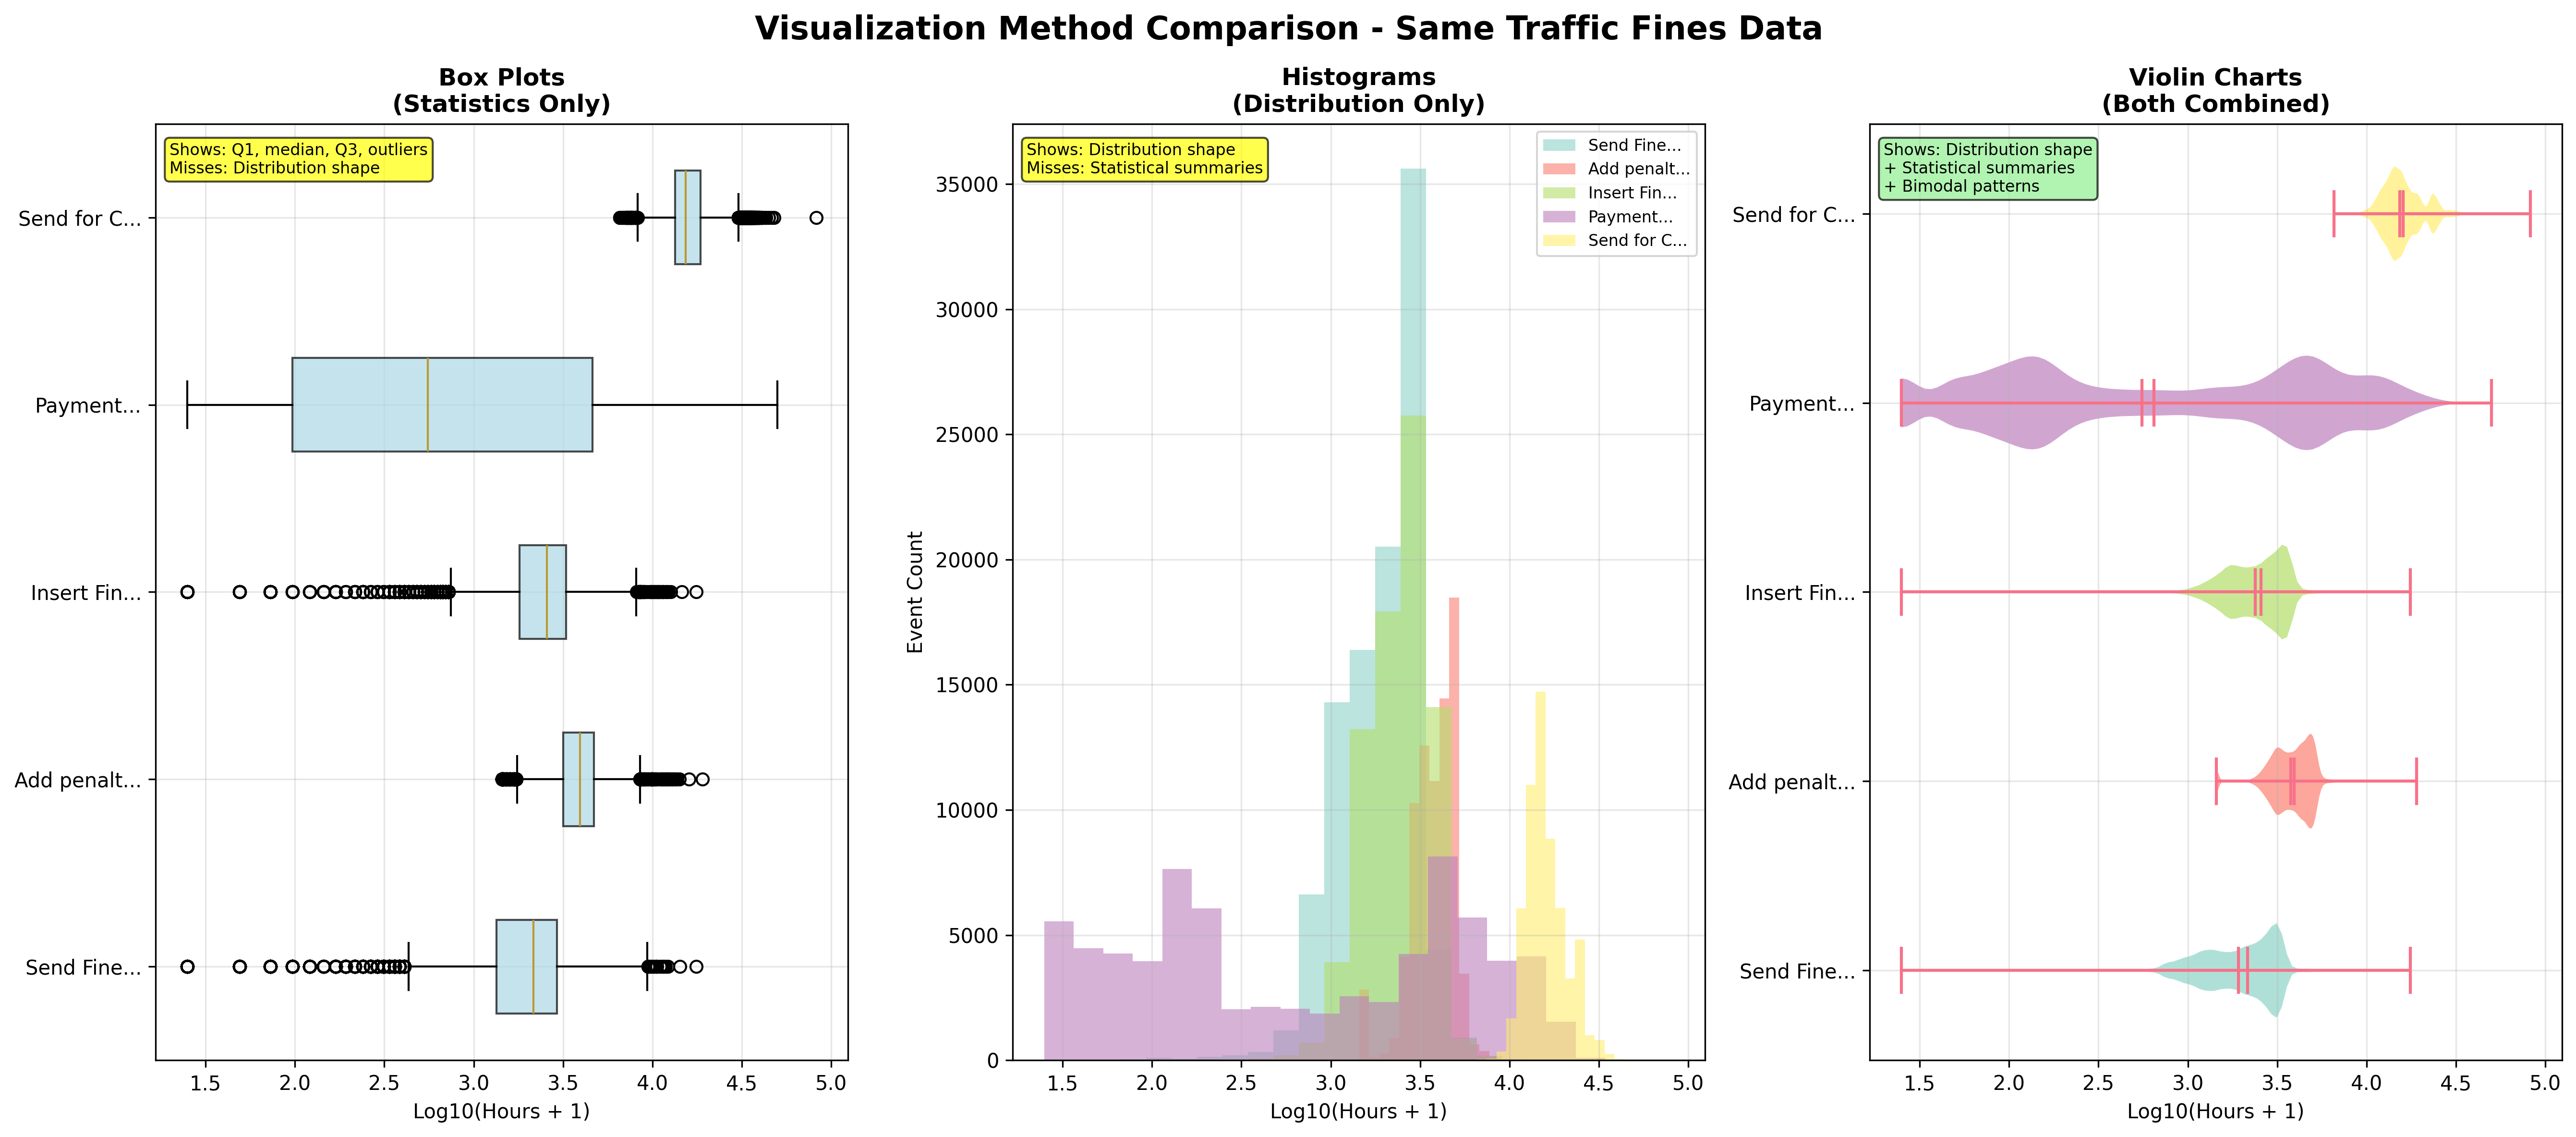
\includegraphics[width=\textwidth]{fig/violin_vs_traditional.png}
\caption{Comparison of visualization methods for the same Traffic Fines data. Box plots show statistical summaries but miss distribution shape, histograms show distribution but hide statistics, while violin charts integrate both perspectives to reveal bimodal patterns and statistical summaries simultaneously.}
\label{fig:violin_vs_traditional}
\end{figure}

\textbf{Multimodal Patterns:} Traffic Fines showed clear bimodal distributions indicating two distinct citizen behavior patterns (immediate vs delayed payment), information lost in box plots or histograms.

\textbf{Distribution Shapes:} Healthcare processes exhibited left-skewed distributions reflecting urgent care protocols, while financial processes showed right-skewed patterns indicating processing delays.

\textbf{Statistical Integration:} Simultaneous display of distribution shape and statistical summaries enabled comprehensive analysis without switching between multiple chart types.

\textbf{Interactive Exploration:} Different statistical sorting revealed complementary insights - frequency sorting identified common events while mean sorting revealed typical timing patterns, as shown in Figure \ref{fig:sorting_effects}.

\begin{figure}[H]
\centering
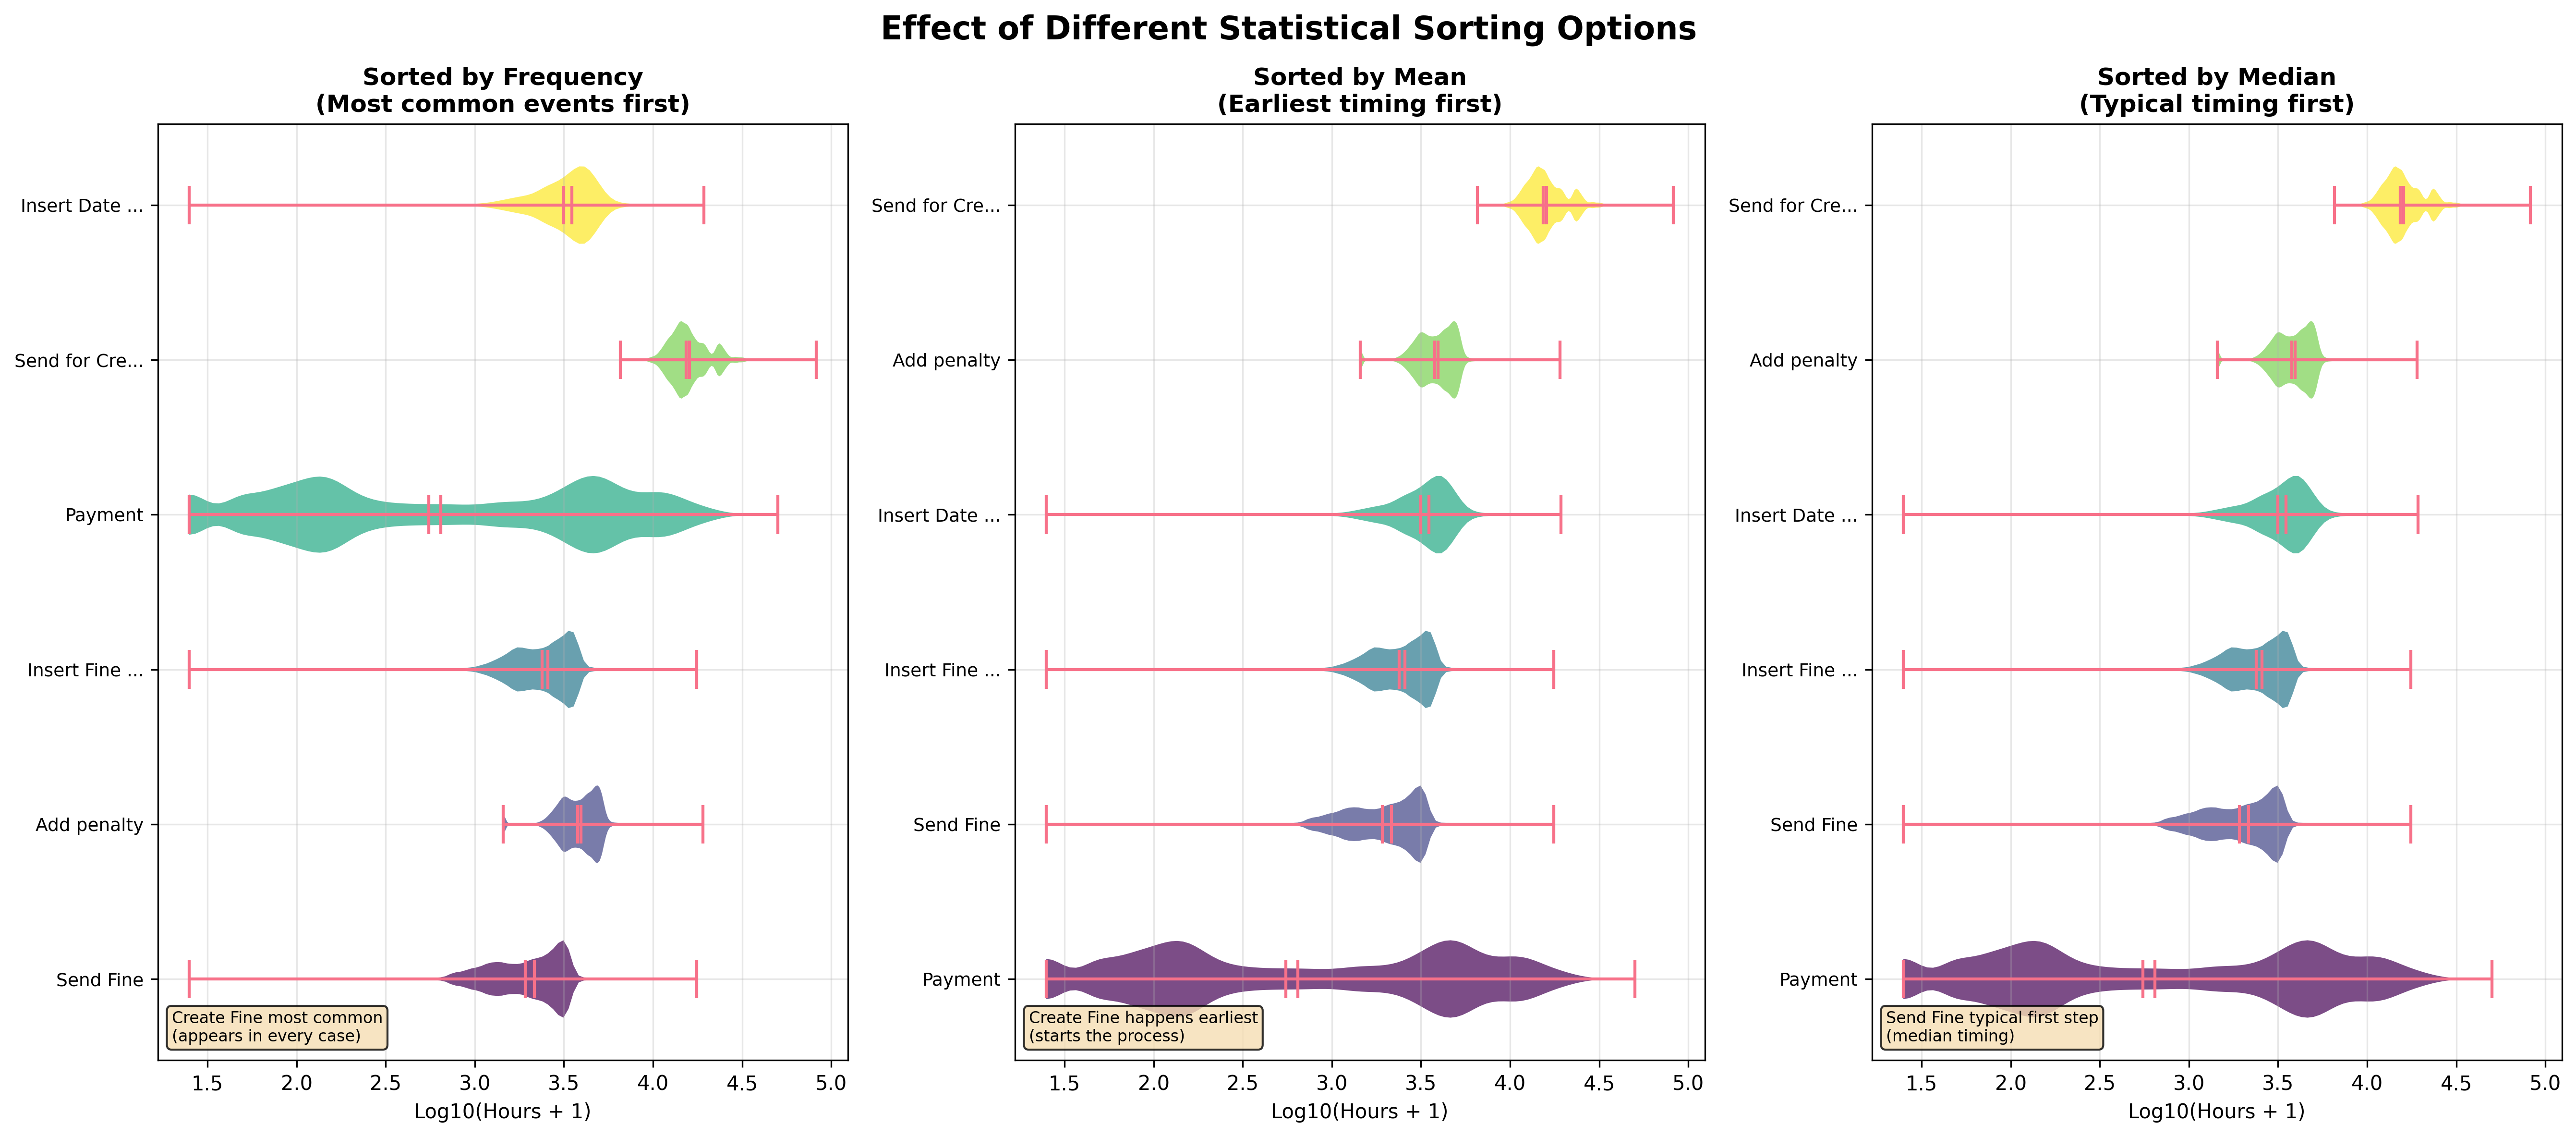
\includegraphics[width=\textwidth]{fig/sorting_effects.png}
\caption{Effect of different statistical sorting options on event ordering. Frequency sorting reveals the most common events, mean sorting shows which events typically occur early or late, and median sorting highlights typical timing patterns. Each perspective provides different analytical insights from the same data.}
\label{fig:sorting_effects}
\end{figure}

\subsection{Limitations and Discussion}
\label{subsec:limitations}

Several limitations emerged during evaluation:

\textbf{Sparse Data Handling:} Very sparse distributions with few events can create misleading violin shapes. Our minimum event threshold of 100 occurrences helps but doesn't eliminate this issue.

\textbf{Extreme Outliers:} Despite filtering and transformation, some datasets still contain extreme outliers that can distort visualizations. Manual outlier detection may be needed for certain analyses.

\textbf{Transformation Selection:} Users need domain knowledge to select optimal transformations. Automatic transformation recommendation could improve usability.

\textbf{Scalability Limits:} While tested up to 1.2 million events, performance with datasets exceeding 10 million events remains unknown and may require additional optimization.

Despite these limitations, the approach successfully addresses the core requirements and provides significant improvements over traditional visualization methods for process mining analysis.
